\documentclass[12pt]{report}

\usepackage[utf8]{inputenc}
\usepackage{amsmath}
%\usepackage{ae}
\usepackage{graphicx}
\usepackage{color}
\usepackage{tikz}
\usepackage[tc]{titlepic}

%\usepackage{bbm}
%\usepackage[swedish]{babel}
\newcommand{\N}{\ensuremath{\mathbbm{N}}}
\newcommand{\Z}{\ensuremath{\mathbbm{Z}}}
\newcommand{\Q}{\ensuremath{\mathbbm{Q}}}
\newcommand{\R}{\ensuremath{\mathbbm{R}}}
\newcommand{\C}{\ensuremath{\mathbbm{C}}}
\renewcommand{\d}{\ensuremath{\mathrm{d}}}
\newcommand{\e}{\ensuremath{\mathrm{e}}}
\renewcommand{\L}{\ensuremath{\mathcal{L}}}
\renewcommand{\i}{\ensuremath{i}}
%\renewcommand{\i}{\ensuremath{\mathrm{i}}}
\newcommand{\ket}[1]{|#1\rangle}
\newcommand{\bra}[1]{\langle#1|}
\newcommand{\braket}[2]{\bra{#1}#2\rangle}
\newcommand{\bracket}[3]{\bra{#1}#2\ket{#3}}
\newcommand{\fig}[3]{
\begin{figure}
\centering
\includegraphics{figs/#1}
\caption{#2}
\end{figure}
}


\title{Holographic Superconductivity}
\author{Petter Säterskog}
\begin{document}

\titlepic{
\centering
\begin{tikzpicture}
    \draw[->] (0,3) -- (1,3) node[right] {$z$};
    \draw[-,thick] (0,-1.5) -- (0,4) node[above] {Boundary};
    \draw[-,thick] (6,-1.5) -- (6,4) node[above] {Horizon};
    \draw[-] (6,0) -- (-0.5,0) node[left] {$m_{\mathrm{eff}}^2=0$};
    \draw[-] (6,1) -- (-0.5,1)[dashed] node[left] {$m_{\mathrm{eff}}^2=m^2$};
    \draw[-] (6,-1) -- (-0.5,-1)[dashed] node[left] {BF bound};
    \draw[dotted] plot[domain=1:0.5,samples=100] (\x*6,{4*(1-\x)})node[above] {$\phi$};
    \draw[-] (6,0) node[right] {$\phi=0$, $\phi^\prime>0$};
    \draw[solid] plot[domain=0:1,samples=100] (\x*6,{1-2*\x*\x/(1-\x*\x*\x)*4*(1-\x)*4*(1-\x)});
\end{tikzpicture}
}
\maketitle
\tableofcontents
\chapter{Introduction}
The AdS-CFT correspondence was conjectured in 1997 \cite{Maldacena:1997re}. It relates the physics of a string theory in Anti de Sitter space (AdS) to a conformal field theory (CFT) on the boundary of the AdS space.

Strong coupling

High TC Superconductors
\section{The Correspondence}
The correspondence can be formulated by the GKPW equation \cite{Witten:1998qj}
\begin{equation}
 Z_{\text{CFT}}=Z_{\text{strings}}
\label{GKPW}
\end{equation}
where $Z_{\text{CFT}}$ is the partition function of the boundary theory and $Z_{\text{strings}}$ is the partition function of the bulk theory. The relation between the Lagrangians of the theories is unknown but the boundary values of fields in the bulk theory correspond to fields in the CFT.
\section{Restrictions}
Lorentz invariance, relativity, causality, locality?
\section{Partition Function}
The partition function is a concept from statistical physics. It is for a quantum-mechanical system defined as
\begin{equation}
 Z(\beta)=\mathrm{tr}(\e^{-\beta\hat{H}})
\end{equation}
where $\hat{H}$ is the time independent Hamiltonian and $\beta=(k_BT)^{-1}$ where $k_B$ is Boltzmann's constant and $T$ is the temperature. Hereafter we let $k_B=1$ meaning that we measure temperature in units of what energy it corresponds to. This is similar to the trace of the time-evolution operator $\hat{U}(t_2,t_1)$ evolving a state from time $t_1$ to $t_2$
\begin{equation}
 \mathrm{tr}(\hat{U}(t_2,t_1))=\mathrm{tr}(\e^{-\i\frac{(t_2-t_1)\hat{H}}{\hbar}})=f(t_2-t_1).
\end{equation}
We will hereafter let $\hbar=1$ by measuring energy in units of inverse time. The partition function can then be obtained as the analytical extension of $f$,
\begin{equation}
 Z(\beta)=f(-\i\beta).
\end{equation}
The trace of the time evolution operator can be calculated as an integral over configuration space which in our case will be fields configurations $\psi$,
\begin{equation}
 f(t)=\int \mathcal{D}[\psi] \bracket{\psi}{\hat{U}(t,0)}{\psi}.
\end{equation}
The time-evolution operator can be calculated using Feynman's path integrals \cite{feynman1965quantum},
\begin{equation}
 \bracket{\psi_2}{\hat{U}(t,0)}{\psi_1}=\int_{\psi_1}^{\psi_2} \mathcal{D}[\psi(t)]\e^{\i S[\psi(t)]}
\end{equation}
where $S[\psi(t)]$ is the action of the path through field configurations $\psi(t)$. Combining these results tells us that the trace $f(t)$ can be calculated as a periodic time path integral with period $t$
\begin{equation}
 f(t)=\int_0^t \mathcal{D}[\psi(t)]\e^{\i S[\psi(t)]}.
\end{equation}
This means that $Z(\beta)$ can be obtained by calculating a path integral where the time is imaginary and periodic. The action must be analytically extended to imaginary time $\tau=\i t$.
\begin{equation}
 S[x(\tau)]=\int_0^\beta\d \tau \L
\end{equation}
The CFT we are interested in lives on the boundary of an AdS theory. The metric of the CFT is the metric induced from the bulk theory. The boundary is time-like and the time periodicity of the two theories are thus the same. This means that they are at the same temperatures.\\
Only paths of extremal action will contribute to this in the classical limit because of the oscillatory behaviour of the exponential. Let $\psi_\mathrm{c}(t)$ be the path that extremizes the action and expand the exponent as a Taylor series around this
\begin{equation}
\begin{split}
 S[\psi_\mathrm{c}(t)+\psi(t)]=S[\psi_\mathrm{c}(t)]+\frac{\psi(t)^2}{2!}\frac{\delta^2}{\delta\psi(t)^2} S[\psi_\mathrm{c}(t)]+
\frac{\partial_t\psi(t)^2}{2!}\frac{\delta^2}{\delta(\partial_t\psi(t))^2} S[\psi_\mathrm{c}(t)]+O(\psi(t)^3)
\end{split}
\end{equation}
The functional derivative of the action is just the ordinary derivative of the Lagrangian function. TODO
The partition function is in the classical limit
\begin{equation}
 Z(\beta)=f(-\i\beta)\stackrel{\mathrm{classical}}{=} \e^{i S_c}\label{classical}
\end{equation}
where $S_c$ is the action of classical periodic path with period $-\i\beta$.
\section{Expectation Values}
The boundary values of the bulk fields correspond to fields in the CFT. Expectation values of observables in the CFT can be calculated using a generating functional $Z[J]$. This is a partition function for a system with a perturbed Lagrangian $\L_J(x)=\L(x)+J(x)O(x)$. Here $O(x)$ is a local operator on the fields. The generating functional can be regarded an expectation value of a system with the original Lagrangian $\L$.
\begin{equation}
\begin{split}
 Z[J]&=\int_0^{-\i\beta} \mathcal{D}[\psi(t)]\e^{\i \int \L(\psi(x))+J(x)O(\psi(x))}\\
&=Z[0]\int_0^{-\i\beta} \mathcal{D}[\psi(t)]\frac{\e^{\i\int \L(\psi(x))}}{Z[0]}\e^{\i\int J(x)O(\psi(x))}\\
&=Z[0]\langle\e^{\i\int J(x)O(\psi(x))}\rangle
\end{split}
\end{equation}
Taking a functional derivative of this gives:
\begin{equation}
\begin{split}
 \frac{\delta}{\delta J}\log(Z[J])|_{J=0}&=\frac{Z[0]\langle\i O(\psi(x))\e^{\i\int J(x)O(\psi(x))}\rangle}{  Z[0]\langle\e^{\i \int J(x)O(\psi(x))}\rangle }\big |_{J=0}\\
&=\i \langle O(\psi(x))\rangle\label{expectation}
\end{split}
\end{equation}
The partition functions of the bulk and boundary theories are the same even for a perturbed Lagrangian. Both Lagrangians are then perturbed. Expectation values of operators of the boundary theory can thus be calculated using the partition function for the bulk theory. It is though not trivial to figure out what fields in the bulk theory corresponds to what operators in the boundary theory
\chapter{Solution of the Classical Bulk Theory}
We wish to compute expectation values of the CFT. The field theory is a strongly coupled quantum field theory and the expectation values are thus difficult to compute directly. The expectation values can though be calculated using \eqref{expectation} and the partition function can be obtained from the GKPW equation, \eqref{GKPW}.\\

The partition function of the bulk theory must then be calculated. This is in our case easier, TODO reference, since this theory can be treated in a classical limit. But the equations of motion must still be calculated and the solutions must be translated to expectation values for the CFT. This section is devoted to the theory of how this is done.
\section{Metric}
The precise form of the bulk Lagrangian that corresponds to the boundary theory we are interested in is unknown. The string theory is gravitational and the space is asymptotically AdS. The action contains an Einstein-Hilbert term with a cosmological constant
\begin{equation}
\Lambda=-\frac{d(d-1)}{2L^2}
\end{equation}
where $L$ is a length scale and $d$ is the dimension of the boundary.
A Gibbons-Hawking-York boundary term is also needed \cite{PhysRevD.15.2752}, \cite{PhysRevLett.28.1082} TODO, read, comment.
\begin{equation}
 S_{\mathrm{grav}}=\frac{1}{2\kappa}\int \d^{d+1}x\sqrt{-g}\left(R-2\Lambda\right)-\frac{1}{\kappa}\int \d^dx\sqrt{\gamma}\left(-\gamma^{ab}\nabla_an_b+\frac{d-1}{L}\right)
\end{equation}
Here $R$ is the Ricci scalar. The gravitational constant $\kappa$ (related to Newton's constant by $\kappa=8\pi G$) is assumed to be small so that we are in a so called ``probe limit''. We will later see when this assumption can't be trusted, TODO. $n_a$ is a normal vector at the boundary. The probe limit lets us solve the equations of motion for the metric independently of the other fields. We are looking for an equilibrium solution at a finite temperature $T$ and the solution is then known to be a black hole(TODO ref), the Schwarzschild metric in AdS space. The metric has the following form in a particular choice of coordinates where the radial coordinate $z$ is 0 at the boundary and $z_h$ at the horizon
\begin{equation}
 g_{ab}\d x^a\d x^b=\frac{L^2}{z^2}\left(\frac{\d z^2}{f(z)}-f(z)\d t^2+\d \mathbf{x}^2\right).\label{metric}
\end{equation}
Here $f(z)=1-z^dz_h^{-d}$. The vector $\mathbf{x}$ thus has $d-1$ components. $f(z)$ approaches 1 at the boundary and the space is asymptotically AdS.\\
All coordinates are evidently of the same unit. The gravitational part of the Lagrangian can now be removed and this background metric can be used instead of solving the equations of motion for the metric together with the fields. This gravitational part of the Lagrangian must though be kept when calculating the value of the total action. The Ricci scalar of this metric is
\begin{equation}
 R=-\frac{d(d+1)}{L^2}=2\Lambda\frac{d+1}{d-1}
\end{equation}
TODO: does the region behind the horizon contribute?
The action can be calculated using this. Consider the space $(z,t,\mathbf{x})\in[\epsilon,z_h]\times V$ corresponding to a $d$-volume of the boundary theory $V$. The action boundary density is then
\begin{equation}
\begin{split}
 \frac{S_{\mathrm{grav}}}{V}&=\frac{\Lambda}{\kappa}\left(\frac{d+1}{d-1}-1\right)\int_\epsilon^{z_h}\d z\sqrt{-g}+
\frac{1}{\kappa}\sqrt{\gamma}\left(-\gamma^{ab}\partial_a\d z_b+\frac{d-1}{L}\right)\\
&=\frac{\Lambda}{\kappa}\frac{2}{d-1}\int_\epsilon^{z_h}\d z\left(\frac{L}{z}\right)^{d+1}+
\frac{1}{\kappa}\left(\frac{\epsilon}{L}\right)^{-d}\frac{d-1}{L}\\
&=\frac{L\Lambda}{\kappa}\frac{2}{d(d-1)}\left(\left(\frac{\epsilon}{L}\right)^{-d}-\left(\frac{z}{L}\right)^{-d}\right)\\
&=-\frac{1}{L\kappa}\left(\left(\frac{\epsilon}{L}\right)^{-d}-\left(\frac{z_h}{L}\right)^{-d}\right)
\end{split}
\end{equation}

The total action density is obtained as $\epsilon\rightarrow0$.
.  TODO, imaginary time, deficit angle gives $T$.


\begin{equation}
 T=\frac{d}{4\pi  z_h}\label{T}
\end{equation}
%This $T$ in units of energy is also in units of inverse length since we chose the energy unit to the inverse time it 
\section{Boundary Behaviour}
The bulk Lagrangian considered will contain different fields and depends both on the fields and their first derivatives. Consider a field $\psi$ with a kinetic term $-(\partial_a\psi)^2$ and a potential term $V(\psi)$. The classical solution is the one that extremizes the action. The action integral contains the metric as an integration measure
\begin{equation}
 S=\int\d^{d+1} x\sqrt{|\det g_{ab}|}\L\equiv\int\d^{d+1} x\sqrt{g}\L.
\end{equation}
The Euler-Lagrange equation is obtained by varying the action. The integration measure can then be regarded as part of the Lagrangian or covariant derivatives can be used in the derivation of the Euler-Lagrange equation. The measure becomes when using the metric \eqref{metric} $L^{d+1}z^{-d-1}$. The Euler-Lagrange equation gives
\begin{equation}
\begin{split}
 0=\partial_a\left(\frac{\partial (z^{-d-1}(V(\psi)-(\partial_b\psi)^2)) }{\partial(\partial_a\phi)}\right)-\frac{\partial  (z^{-d-1}(V(\psi)-(\partial_b\psi)^2) )}{\partial\phi}=\\
 =-\partial_a\left(z^{-d-1}2\partial^a\psi\right)-z^{-d-1}V'(\psi)\\
\end{split}
\end{equation}
We will be interested in boundary systems with translational symmetry so $\psi$ is assumed to be a function of $z$, TODO motivate more. The equation of motion then becomes
\begin{equation}
\begin{split}
0=-\partial_z\left(z^{-d-1}2g^{zz}\partial_z\psi\right)  -\frac{V'(\psi)}{z^{d+1}}=\\
-\partial_z\left(z^{-d-1}2(z^2L^{-2}f(z))\partial_z\psi\right)  -\frac{V'(\psi)}{z^{d+1}}=\\
-z^{-d-1}2z^2L^{-2}f(z)\psi''-L^{-2}\left((-d+1)z^{-d}2f(z) + z^{-d+1}2f'(z)\right)\psi' -\frac{V'(\psi)}{z^{d+1}}
\end{split}
\end{equation}
This gives a second order differential equation for $\psi(z)$
\begin{equation}
\begin{split}
0=-z^22f(z)\psi''-\left((-d+1)z2f(z) + z^22f'(z)\right)\psi' -L^2V'(\psi)
\end{split}
\end{equation}
Now consider the boundary, $z=0$. Our metric is required to be asymptotically AdS so $f(0)\rightarrow1, zf'(0)\rightarrow0$. $\psi$ can be expanded at the boundary as a Laurent series. Call the lowest exponent in this series $\Delta$. $\psi$ will then behave as $z^\Delta$ near the boundary. This should solve the differential equation in the near boundary limit. Insertion of $z^\Delta$ into the differential equation and taking the limit of small $z$ gives
\begin{equation}
\begin{split}
0&=-z^22\Delta(\Delta-1)z^{\Delta-2}-\left((-d+1)2z + z^22f'(z)\right)\Delta z^{\Delta-1} -L^2V'(z^{\Delta})\\
&=z^{\Delta}\left(-2\Delta(\Delta-1)-2(-d+1)\Delta\right)-L^2V'(z^{\Delta}).
\end{split}
\end{equation}
Now consider a potential for a massive scalar field, $V(\psi)=-m^2\psi^2+\mathcal{O}(\psi^3)$. We then get the following equation for $\Delta$
\begin{equation}
\begin{split}
%0=\Delta(\Delta-1)-(d-1)\Delta-L^2m^2=\\
0=\Delta^2-d\Delta-L^2m^2
\end{split}
\end{equation}
in the limit $z\rightarrow0$. This has solutions
\begin{equation}
\begin{split}
\Delta=\frac{d\pm\sqrt{d^2+4L^2m^2}}{2}.
\end{split}
\end{equation}
$\psi$ thus goes as $z^{\Delta_0}$ where $\Delta_0$ is the smaller solution and $\Delta_1$ the larger. The leading behaviour of $\psi$ near $z=0$ is
\begin{equation}
 \psi=\psi_0\left(\frac{z}{L}\right)^{\Delta_0}+\psi_1\left(\frac{z}{L}\right)^{\Delta_1}
\end{equation}
unless $\Delta_1-\Delta_0>=1$ and further terms from the series corresponding to $\Delta_0$ must be included.\\

What will the contribution to the action from this solution be? Consider the action contribution from the region $z\in[\epsilon,\delta]$ where $\delta$ is small and $\epsilon\rightarrow0$.
\begin{equation}
\begin{split}
 S_{[\epsilon,\delta]}=&\int_{z\in[\epsilon,\delta]}\d^{d+1} x\sqrt{g}\L=\\
=&V\int_\epsilon^\delta\d z \left(\frac{z}{L}\right)^{-d-1}\left(-m^2\psi^2-(\partial_a\psi)^2\right)=\\
=&V\int_\epsilon^\delta\d z \left(\frac{z}{L}\right)^{-d-1}\left(-m^2( \psi_0\left(\frac{z}{L}\right)^{\Delta_0}+\psi_1\left(\frac{z}{L}\right)^{\Delta_1} )^2-(\partial_a(\psi_0\left(\frac{z}{L}\right)^{\Delta_0}+\psi_1\left(\frac{z}{L}\right)^{\Delta_1}))^2\right)=\\
=&V\int_\epsilon^\delta\d z \left(\frac{z}{L}\right)^{-d-1}\Big[-m^2 \left(\psi_0^2\left(\frac{z}{L}\right)^{2\Delta_0}+\psi_1^2\left(\frac{z}{L}\right)^{2\Delta_1}+2\psi_0\psi_1\left(\frac{z}{L}\right)^{\Delta_0+\Delta_1}\right) \\
&-g^{zz}L^{-2}(\Delta_0\psi_0\left(\frac{z}{L}\right)^{\Delta_0-1}+\Delta_1\psi_1\left(\frac{z}{L}\right)^{\Delta_1-1})^2\Big]=\\
=&V\int_\epsilon^\delta\d z\left(\frac{z}{L}\right)^{-d-1}\Big[-m^2 \left(\psi_0^2\left(\frac{z}{L}\right)^{2\Delta_0}+\psi_1^2\left(\frac{z}{L}\right)^{2\Delta_1}+2\psi_0\psi_1\left(\frac{z}{L}\right)^{\Delta_0+\Delta_1}\right)\\
&-g^{zz}L^{-2}\left(\Delta_0^2\psi_0^2\left(\frac{z}{L}\right)^{2(\Delta_0-1)}+\Delta_1^2\psi_1^2\left(\frac{z}{L}\right)^{2(\Delta_1-1)}+
2\Delta_0\Delta_1\psi_0\psi_1\left(\frac{z}{L}\right)^{\Delta_0+\Delta_1-2}\right)\Big]=\\
=&V\int_\epsilon^\delta\d z\Big[-m^2 \left(\psi_0^2\left(\frac{z}{L}\right)^{2\Delta_0-d-1}+\psi_1^2\left(\frac{z}{L}\right)^{2\Delta_1-d-1}+2\psi_0\psi_1\left(\frac{z}{L}\right)^{-1}\right)\\
&-L^{-2}\left(\Delta_0^2\psi_0^2\left(\frac{z}{L}\right)^{2\Delta_0-d-1}+\Delta_1^2\psi_1^2\left(\frac{z}{L}\right)^{2\Delta_1-d-1}-
2L^2m^2\psi_0\psi_1\left(\frac{z}{L}\right)^{-1}\right)\Big]=\\
=&V\int_\epsilon^\delta\d z \left((-m^2-\Delta_0^2L^{-2})\psi_0^2\left(\frac{z}{L}\right)^{2\Delta_0-d-1}+(-m^2-\Delta_1^2L^{-2})\psi_1^2\left(\frac{z}{L}\right)^{2\Delta_1-d-1}\right)=\\
=&VL^{-2}(\Delta_1-\Delta_0)\int_\epsilon^\delta\d z \left(\Delta_0\psi_0^2\left(\frac{z}{L}\right)^{2\Delta_0-d-1}-\Delta_1\psi_1^2\left(\frac{z}{L}\right)^{2\Delta_1-d-1}\right)=\\
=&VL^{-1}(\Delta_1-\Delta_0)\left(-\frac{ \Delta_0\psi_0^2}{2\Delta_0-d}\left(\frac{\epsilon}{L}\right)^{2\Delta_0-d}+
\frac{\Delta_1 \psi_1^2}{2\Delta_1-d}\left(\frac{\epsilon}{L}\right)^{d-2\Delta_0}\right)+\mathrm{finite}\\
=&VL^{-1}\left(\Delta_0\psi_0^2\left(\frac{\epsilon}{L}\right)^{2\Delta_0-d}-
\Delta_1\psi_1^2\left(\frac{\epsilon}{L}\right)^{d-2\Delta_0}\right)+\mathrm{finite}
\end{split}
\end{equation}
Here $\Delta_0+\Delta_1=d$ and $\Delta_0\Delta_1=-L^2m^2$ have been used. One of these two terms diverges as $\epsilon\rightarrow0$. The term with $\psi_0$ diverges since $2\Delta_0-d=-\sqrt{d^2+4L^2m^2}$. The action from the near boundary thus diverges. This can be remedied by having a boundary term in the action that exactly cancels this divergence.\\
The boundary term must thus evaluate to
\begin{equation}
-\Delta_0VL^{-1}\psi_0^2\left(\frac{\epsilon}{L}\right)^{2\Delta_0-d}
\end{equation}
near the boundary. A boundary term like this can be constructed using $\psi=\psi_0L^{-\Delta_0}\epsilon^{\Delta_0}$ near the boundary and $\sqrt{\gamma}=L^dz^{-d}$ where $\gamma$ is the determinant of the metric induced on the boundary by $g_{ab}$.
The boundary term then becomes
\begin{equation}
\begin{split}
 S_{\mathrm{bdy}}&=-\int_{z=\epsilon}\d^dx\Delta_0L^{-1}\psi^2\sqrt{\gamma}
\label{Sbdy}
\end{split}
\end{equation}
This is addition to the Lagrangian is Lorentz invariant and it also has conformal invariance.
\\
Consider another possible term in the Lagrangian, an electromagnetic field $A_\mu$. The Lagrangian is $-\frac{1}{4}F_{ab}F^{ab}$ where $F_{ab}=\partial_aA_b-\partial_bA_a$. Consider fields with $t$, $x_1$, and $x_2$ symmetry.
\\
TODO, check. It is easily shown that the behaviour of these fields is the same when there is an interaction present as will be considered later.
\section{Horizon Beaviour}
TODO: Wilson loop=>$\phi=0$. Ingoing boundary conditions.
Looking at the equations of motion for $z\rightarrow z_h$ gives when $\phi(z_h)=0$
\begin{equation}
 \psi(z_h)=\frac{-3z_h\psi^\prime(z_h)}{L^2m^2}
\end{equation}

\section{Expectation Values of Boundary Operators}
These expectation values are calculated using \eqref{expectation} and \eqref{classical}.
\begin{equation}
\begin{split}
\langle O(\psi(x))\rangle=-i\frac{\delta}{\delta J(x)}\log(Z[J])|_{J=0}\stackrel{\mathrm{GKPW}}{=}-i\frac{\delta}{\delta J(x)}\log(Z[J])|_{J=0}\stackrel{\mathrm{classical}}{=}\frac{\delta}{\delta J(x)}S_c|_{J=0}
\end{split}
\end{equation}
The functional derivative is thus the change in the classical action when the boundary value of the fields are changed. The total change in the partition function is needed and the whole field solutions change when changing the boundary conditions so this must be taken into account. The derivative becomes
\begin{equation}
\begin{split}
\frac{\delta}{\delta J(x)}S_c|_{J=0}=\int \d^{d+1}y\sqrt{g}\left(\frac{\partial\L(y)}{\partial \phi_i(y)}\frac{\partial \phi_i(y)}{\partial J(x)}+\frac{\partial\L(y)}{\partial (\partial_a\phi_i(y))}\frac{\partial (\partial_a\phi_i(y))}{\partial J(x)}\right)
\end{split}
\end{equation}
where $i$ goes over all fields. Here the Lagrangian is assumed to only depend on the fields and their first derivatives. Now let $\L^\prime=\sqrt{g}\L$ and integrate by parts
\begin{equation}
\begin{split}
\frac{\delta}{\delta J(x)}S_c|=&\int \d^{d+1}y\left(\frac{\partial\L^\prime(y)}{\partial \phi_i(y)}-\partial_a\frac{\partial\L^\prime(y)}{\partial (\partial_a\phi_i(y))}\right)\frac{\partial (\phi_i(y))}{\partial J(x)}\\
+&\int_{\partial\mathrm{AdS}} \d^{d}yn_a\frac{\partial\L^\prime(y)}{\partial (\partial_a\phi_i(y))}\frac{\partial (\phi_i(y))}{\partial J(x)}
\end{split}
\end{equation}
where $n_a$ is an outward normal to the boundary of AdS.
The first integral vanishes since the fields obey the Euler-Lagrange equation.
\chapter{Application to Two-Dimensional Electron Condensates}
TODO, Strong coupling, classical limit.
TODO, motivate, reference. The Lagrangian used is
\begin{eqnarray}
 \mathcal{L}=&\frac{1}{2\kappa}\left(R-2\Lambda\right)-\frac{1}{4}F_{ab}F^{ab}-m^2\psi\overline{\psi}-D_a\psi\overline{D^a\psi}
+\gamma C_{abcd}F^{ab}F^{cd}\nonumber\\
&+\alpha_1(F_{ab}F^{ab})^2+\alpha_2F^a_bF^b_cF^c_dF^d_a
\end{eqnarray}
TODO, describe term by term.
The first term is an Einstein-Hilbert term with a cosmological constant $\Lambda$.
where $D_a$ is the gauge covariant derivative $D_a=\nabla_a-iqA_a$ and $F_{ab}=\partial_aA_b-\partial_bA_a$. This Lagrangian is invariant under a U(1) gauge transformation
\begin{eqnarray}
 \psi&\rightarrow&\mathrm{e}^{i\theta(x)}\psi\\
 A_a&\rightarrow& A_a+\frac{1}{q}\nabla_a\theta(x).
\end{eqnarray}
This lets us make a choice of gauge, $\nabla_aA^a=0$, the Lorentz gauge. The gauge is still not completely fixed, a gauge transformation $\theta(x)$ such that $\nabla_a\nabla^a\theta(x)=0$ can still be done without violating the gauge condition.
The Lagrangian is also evidently Lorentz invariant imposing Lorentz invariance of the boundary theory. This Lagrangian also posseses conformal invariance. This means that the Lagrangian is unchanged by the transformation $g_{ab}\rightarrow f(x)g_{ab}$.
\section{Symmetry Assumptions}
\section{Equations of motion}
Describe why $\psi$ can be considered real.\\
First consider a system with $A_r=A_x=A_y=0$. The field equations obtained by varying the fields $\psi$, $\phi$ are respectively
\begin{eqnarray}
0=&\psi \left(- \frac{m^{2}}{\operatorname{f}\left(r\right)} + \frac{\phi^{2}}{\operatorname{f}^{2}\left(r\right)}\right) + \frac{\partial^{2}}{\partial^{2} r}  \psi\nonumber\\&+\left(\frac{\frac{\partial}{\partial r} \operatorname{f}\left(r\right)}{\operatorname{f}\left(r\right)} + \frac{2}{r}\right) \frac{\partial}{\partial r} \psi
\end{eqnarray}
\begin{eqnarray}
0=&- 2 \frac{\phi \psi^{2} r^{2}}{\operatorname{f}\left(r\right)} + r^{2} \frac{\partial^{2}}{\partial^{2} r}  \phi + 2 r \frac{\partial}{\partial r} \phi.
\end{eqnarray}
TODO, boundary conditions.\\
These equations have the trivial solution
\begin{equation}
 \begin{split}
  \psi=&0\\
  \phi=\mu-\mu\frac{z}{z_h}\label{trivial}
 \end{split}
\end{equation}
\section{Parameters}
There are multiple unknown parameters. These must be investigated to find values that give us the boundary theory we are interested in. The Lagrangian contains the parameters $\kappa$, $L$, $m^2$, $q$, $\alpha_1$, $\alpha_2$, and $\gamma$. The solution of the equations of motion for the metric we used in the probe limit also contains a temperature dependent constant $z_h$. Some of these parameters might be redundant since we can make different transformations of fields and coordinates. The physics of the bulk are treated in the classical limit and the Lagrangian can thus be changed as long as the equations of motion for $\psi$ and $A_a$ are left unchanged. The physics are independent of the exact value of $\kappa$ as long as we are in the probe limit.\\

The horizon $z_h$ and the curvature length $L$ set length scales in the metric. Length units in the numerical solution can be chosen such that $z_h=1$. This means that we for different temperatures have different units since $z_h$ is related to the temperature. We will have to convert between these units when comparing results from different temperatures.\\

The factor $L^2$ in the metric does not affect the theory since the Lagrangian has conformal invariance. TODO, true? Let $L=1$ hereafter.\\

Considering $q\psi$ and $qA_a$ as the fields gives a Lagrangian of the same form but with different constants $\alpha_1$, $\alpha_2$, and $\gamma$ and the whole Lagrangian is divided by $q^2$ except for the term originally containing $q^2$ which is divided by $q^4$. Multiplying the Lagrangian by a constant doesn't affect the equations of motion so $q=1$ can be assumed without getting a less general Lagrangian. It should be noted that a different value of $q$ would give $q\psi$ as solution instead where $\psi$ is the solution of the equations of motion when $q=1$. The same is true for $A_a$.\\

%The parameters $\alpha_1, \alpha_2, \gamma$ are dimension-less and can not be scaled away. 
The Breitenlohner-Freedman bound (BF) is a lower bound on $m^2$ of a massive scalar field in AdS space. It requires
\begin{equation}
 L^2m^2\geq-\frac{d^2}{4}\label{BF}
\end{equation}
for stability\cite{Kleban:2004bv}, TODO explain. The scalar field $\psi$ should obey this bound far away from the black-hole for normalizeable modes, TODO explain. We would though like a symmetry breaking of $\psi$ near the black hole corresponding to the electron condensate \cite{Gubser:2008px}. This can happen because the coupling of $\psi$ to $A_a$ gives $\psi$ an effective mass. \\The effective mass is given by:
\begin{equation}
 m_{eff}^2=m^2+A_aA^a
%=m^2+g^{tt}\phi^2
=m^2-\frac{z^2}{L^2(1-z^dz_h^{-d})}\phi^2
\end{equation}

\begin{figure}
\centering
\begin{tikzpicture}
    \draw[->] (0,3) -- (1,3) node[right] {$z$};
    \draw[-,thick] (0,-1.5) -- (0,4) node[above] {Boundary};
    \draw[-,thick] (6,-1.5) -- (6,4) node[above] {Horizon};
    \draw[-] (6,0) -- (-0.5,0) node[left] {$m_{\mathrm{eff}}^2=0$};
    \draw[-] (6,1) -- (-0.5,1)[dashed] node[left] {$m_{\mathrm{eff}}^2=m^2$};
    \draw[-] (6,-1) -- (-0.5,-1)[dashed] node[left] {BF bound};
    \draw[dotted] plot[domain=1:0.5,samples=100] (\x*6,{2*(1-\x)/((1-\x)/2+0.1)})node[above] {$\phi$};
    \draw[-] (6,0) node[right] {$\phi=0$, $\phi^\prime>0$};
    \draw[solid] plot[domain=0:1,samples=100] (\x*6,{1-2*\x*\x*(1-\x)/((1-\x)/2+0.1)*(1-\x)/((1-\x)/2+0.1)/(1-\x*\x*\x)});
\end{tikzpicture}
\caption{Schematic plot of how the the effective mass breaks the BF bound outside the horizon. A value of $\phi$ has been assumed.}
\end{figure}

\begin{figure}
\centering
\begin{tikzpicture}
    \draw[->] (0,3) -- (1,3) node[right] {$z$};
    \draw[-,thick] (0,-1.5) -- (0,4) node[above] {Boundary};
    \draw[-,thick] (6,-1.5) -- (6,4) node[above] {Horizon};
    \draw[-] (6,0) -- (-0.5,0) node[left] {$m_{\mathrm{eff}}^2=0$};
    \draw[-] (6,1) -- (-0.5,1)[dashed] node[left] {$m_{\mathrm{eff}}^2=m^2$};
    \draw[-] (6,-1) -- (-0.5,-1)[dashed] node[left] {BF bound};
    \draw[dotted] plot[domain=1:0.5,samples=100] (\x*6,{4*(1-\x)})node[above] {$\phi$};
    \draw[-] (6,0) node[right] {$\phi=0$, $\phi^\prime>0$};
    \draw[solid] plot[domain=0:1,samples=100] (\x*6,{1-2*\x*\x/(1-\x*\x*\x)*4*(1-\x)*4*(1-\x)});
\end{tikzpicture}
\caption{Schematic plot of how the the effective mass breaks the BF bound outside the horizon. A value of $\phi$ has been assumed.}
\end{figure}

The bulk field equations are obtained by varying the bulk Lagrangian with respect to all the fields. This can be done with the Euler-Lagrange equation since the action does not contain any higher derivatives. The Euler-Lagrange equation for a scalar field $\phi$ states
\begin{equation}
 \partial_a\left(\frac{\partial\mathcal{L}}{\partial(\partial_a\phi)}\right)-\frac{\partial\mathcal{L}}{\partial\phi}.
\end{equation}
$\phi$ is 0 at the horizon but increases as $\psi$ is non-zero. This effective mass breaks the BF bound since $g^{tt}$ diverges at the horizon. TODO, talk to Ulf and do calculations.
{\bf Skip the following?}:\\
Our space, \eqref{metric}, is asymptotically AdS with $d=3$ at the boundary. But what happens near the horizon? Let $s=z_h-z$. Expand $f(z_h-s)$ around $s=0$.
\begin{equation}
 f(z_h-s)%=1-(z_h-s)^{d}z_h^{-d}
=d\frac{s}{z_h}+O(s^2z_h^{-2})
\end{equation}
The metric now becomes
\begin{equation}
\begin{split}
 g_{ab}\d x^a\d x^b&=\frac{L^2}{(z_h-s)^2}\left(\frac{\d s^2}{d\frac{s}{z_h}}-d\frac{s}{z_h}\d t^2+\d \mathbf{x}^2\right)\\
&=\frac{L^2}{z_h^2}\left(\frac{z_h\d s^2}{ds}-\frac{ds\d t^2}{z_h}+\d \mathbf{x}^2\right)
\end{split}
\end{equation}
\\
Summary, fields, parameters, units
\section{Thermodynamic Variables}

The free energy, $A=-T\log{Z}$, is through the GKPW equation the same for the bulk and the boundary theory. This can be calculated in the classical limit in the bulk.
\begin{equation}
 A=-T\log{Z}\stackrel{\mathrm{classical}}{=}-\i T S_c
\end{equation}
Here $S_c$ is the classical periodic time action. The classical field solutions only depend on the $z$ coordinate and are thus proportional to $V=-\i\beta V_2$ where $V_2$ is the area considered in coordinats $x_1$, $x_2$. This gives the free energy per surface area
\begin{equation}
 \frac{A}{V_2}=-\int_0^{z_h}\d z \sqrt{-g}\L+V^{-1}S_{\mathrm{bdy}}
\end{equation}
Consider the case where $m^2=-2$. Then $\Delta_0=1$ and the boundary term is given by \eqref{Sbdy}.\\
\subsection{Gravitational Free Energy}
The action is dominated by the gravitational part since we are in the probe limit. 
The expression for the temperature \eqref{T} can be used to calculate the free energy from the action at finite temperature
\begin{equation}
\begin{split}
 \frac{A_\mathrm{grav}}{V_2}&=-T\frac{-1}{\kappa}\sqrt{\frac{-2\Lambda}{d(d-1)}}\left(\frac{d}{4\pi TL}\right)^{-d}\\
&=\frac{(4\pi)^dT^dL^{d-1}}{d^{d}\kappa}
\end{split}
\end{equation}
\\
The entropy $H$ can now be calculated from the free energy
\begin{equation}
 H=-\frac{\partial A}{\partial T}=-\frac{(4\pi)^dT^{d-1}L^{d-1}}{d^{d-1}\kappa}.
\end{equation}
TODO, Beckenstein-Hawking
\subsection{Free Energy of Scalar and Electromagnetic Fields}
It is important to calculate the free energy not only of the gravitational part of the Lagrangian since we have multiple solutions of the field equations and boundary values at the same temperature. Which solution is physical can be found by finding the one of lowest free energy. Here we neglect the contribution from any back-reaction on the metric. The back-reaction is small since $\kappa$ is small but a small $\kappa$ also makes the effect of the back-reaction on the free energy large. TODO, motivate or say that we leave this open.\\

The free energy of the trivial solution \eqref{trivial} can be found analytically. For this solution we have
\begin{equation}
 \begin{split}
  \psi&=0\\
  \psi'&=0\\
  \phi&=\mu-\mu\left(\frac{z}{z_h}\right)^{d-2}\\
  \phi'&=-(d-2)\frac{\mu}{z_h}\left(\frac{z}{z_h}\right)^{d-3}
 \end{split}
\end{equation}TODO, explain d-3
\begin{equation}
\begin{split}
 \frac{A}{V_\mathrm{SC}}=&-\int_0^{z_h}\d z \sqrt{-g}\L+V_\mathrm{SC}^{-1}S_{\mathrm{bdy}}\\
=&\int_0^{z_h}\d z \left(\frac{z}{L}\right)^{-d-1}\frac{1}{4}F_{ab}F^{ab}\\
=&\int_0^{z_h}\d z \left(\frac{z}{L}\right)^{-d-1}\frac{1}{2}F_{zt}^2g^{zz}g^{tt}\\
=&-\int_0^{z_h}\d z \left(\frac{z}{L}\right)^{-d-1+4}\left(\frac{z}{z_h}\right)^{2(d-3)}(d-2)^2\frac{\mu^2}{2z_h^2}\\
=&-L^{d-3}z_h^{-2d+4}(d-2)^2\frac{\mu^2}{2} \int_0^{z_h}\d z z^{d-3}\\
=&-L^{d-3}z_h^{-d+2}(d-2)\frac{\mu^2}{2}\\
=&-L^{d-3}\left(\frac{4\pi T}{d}\right)^{d-2}(d-2)\frac{\mu^2}{2}
\end{split}
\end{equation}
\fig{A}{Curves corresponding to different solutions at the same temperature. The trivial solution is shown as the thick solid line. The other curves correspond to numerical solutions. The lowest one corresponds to the first root and the other roots follow in order.\label{f:mu}}

\section{Operator Expectation Values}
TODO, introduce $\rho$, $\mu$...
The charge density $\rho$ of the trivial solution \eqref{trivial} is through \eqref{opExp} given by
\begin{equation}
 \rho=\frac{\mu}{z_h}.
\end{equation}
The chemical potential of the trivial solution can thus be calculated given the temperature and charge density
\begin{equation}
 \mu=\frac{d\rho}{4\pi T}.
\end{equation}
The chemical potential of the numerical solutions can be obtained from the boundary values. The result is seen in Fig. \ref{f:mu}.

\fig{muTzeros}{Curves corresponding to different solutions at the same temperature. The trivial solution is shown as the thick solid line. The other curves correspond to numerical solutions. The lowest one corresponds to the first root and the other roots follow in order.\label{f:mu}}

\section{Conductivity}
\chapter{Numerical Solution of Bulk Equations of Motion}
\section{Condensate}
TODO, write in more detail. TODO, write in some clear way about the dimensionless quantities.
The $\psi$ condensate should be obtained without any source. Boundary conditions without source, $\psi_i=0$, are chosen at the boundary. $\psi_1$, $\mu$, and $\rho$ are then unknown. The boundary condition that $\phi=0$ at the horizon is actually a double boundary condition due to the singular form of the equations of motion there. There are thus only two free parameters and it is easiest to start integrating from there. A numerical integrator is used to integrate from the horizon to the boundary. The source term is read off and the horizon conditions are adapted until the source term is zero. This leaves a one dimensional space of solutions since we have two parameters to vary at the horizon but just one constraint on the boundary. $\mu$, $\rho$ and $\epsilon_{ij}\psi_j$ can be read of at the boundary.\\

The fields all have the unit of inverse length and $\rho$ thus has unit inverse length squared. Solutions can be obtained at any temperature by choosing different values of $z_h$. The temperature can be chosen such that the charge density $\rho$ is constant for all solutions. The numerical solution gives $\rho z_h^2$. Choosing a constant $\rho=1$ gives $z_h$ and thus the temperature. We call the highest temperature obtained $T_c$.

\fig{O2Tzeros}{Curves corresponding to different solutions at the same temperature.}


\begin{figure}
\centering
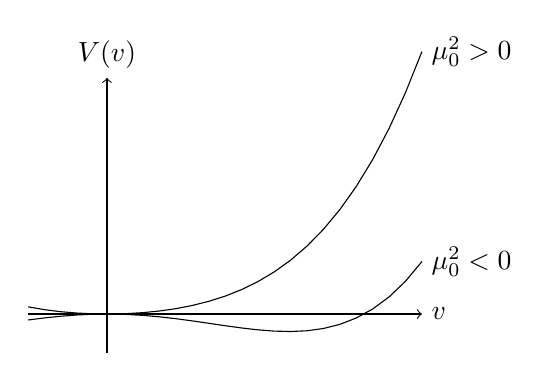
\begin{tikzpicture}
    \draw[->] (-1,0) -- (4,0) node[right] {$v$};
    \draw[->] (0,-0.5) -- (0,3) node[above] {$V(v)$};
    \draw plot[domain=-1:4] (\x,\x*\x*\x*\x/128-\x*\x/12) node[right] {$\mu_0^2<0$};
    \draw plot[domain=-1:4] (\x,\x*\x*\x*\x/128+\x*\x/12) node[right] {$\mu_0^2>0$};
\end{tikzpicture}
\caption{\label{pot}The potential used by Goldstone\cite{McGreevy:2009xe} which also is the Higgs potential. Note the minimum not being at $v=0$ giving a spontaneously broken symmetry.}
\end{figure}

\bibliographystyle{unsrt}
\bibliography{report}
\end{document}